We use the notions of platform and system interchangeably.
We root our platform integration analysis on hardware-software contracts~\cite{guarnieri2021hardware}.
We discuss the relevant scope of observation and execution modes for constant-time verification techniques.
In the light of this discussion, we assess the impact of the spatial scope of the verification and the definition of sinks on the soundness of the verification.
We then formulate \pics that allow to verify constant-time properties in a platform integration context and propose a lightweight CPU instrumentation that augments a CPU with a synthesizable summary of all the potential reentrant information flows from the platform that integrates the CPU.

% \para{Threat model}
% % \fls{Discuss this}
% Understanding desirable requirements regarding  observations requires a threat model definition.
% In this paper, the observer can measure the time taken by a CPU to execute programs when the CPU is integrated in some system, potentially including caches, peripherals or other logic components.
% % \cf{where is the receiver?  if the receiver sees only "program execution time", it isn't clear why monitoring commit timing is insufficient.}
% The observer can however not probe data flows in the system, that is, inside the CPU microarchitecture, between the CPU and the memory, or between the CPU and the I/O devices.
% Physical side-channels are out of scope.
% \fls{TODO Move to its own section.}

\subsection{Observation and execution mode}
\label{subsec:observation_mode}

We have defined in Section~\ref{subsec:non-interference} the notion of observation and execution modes in the context of hardware-software contracts.
The observation mode defines the observable events produced by the ISA execution.
In particular, verification against an observation mode that is weaker than what the design under verification will be subject to when deployed in a system can lead to unsoundness of the verification in the sense that Equation~\ref{eq:microtrace} might hold for a CPU in isolation but not integrated in a system.

\para{Observation mode ordering}
Observation modes define the observable events produced by the ISA execution.
Intuitively, they define what an observer such as a concurrent software thread can learn from the execution of another (victim) thread on the CPU.
They allow software developers to determine if it is safe to use secret data as an input of certain instructions such as multiplications or as memory addresses.
There exists a partial ordering of observation modes~\cite{guarnieri2021hardware}.
An observation mode is stronger than another if for any execution, the set of observable events produced by the latter is a subset of the observable events produced by the former observation mode. 
A stronger observation mode is more discriminative at the ISA level by making Equation~\ref{eq:isatrace} harder to satisfy.
A non-interference contract against a stronger observation mode relaxes requirements on hardware.

\para{The constant-time observation mode}
The original definition of the constant-time~\cite{guarnieri2021hardware} observation mode exposes the program counter (PC) of each executed instruction, the addresses of memory operations, and the operands of variable-latency instructions, with respect to the execution mode.
We argue that this observation mode can be split into two parts.
The sequence of PC values and the operands of variable-latency instructions are observable on a CPU in isolation or connected to any system.
The sequence of memory addresses is observable only when the CPU is integrated into a system where the timing of memory operations depends on the address, and hence this observation mode conservatively assumes that the CPU will be integrated into such a system, for example with a data cache.
As we will discuss, not all the contemporary constant-time verification techniques take into account the potential address-dependent timing effect of components such as caches that are located outside of the CPU under verification~\cite{ceesay2024mucfi,dinesh2024conjunct,dinesh2025h}.
% The motivation for authorizing the observation of addresses of memory operations is that almost all realistic systems will have a behavior or timing that depends on memory addresses.
% For example, a secret might influence whether a present or future memory transaction will hit or miss a cache line, or whether it will affect a memory-mapped element such as a peripheral or an interrupt controller.
% All these secret-dependent behaviors are eventually observable through timing.

\para{Execution mode}
Like explicitly announced in LeaVe~\cite{wang2023specification} and Contract Shadow Logic (CSL)~\cite{tan2025contractshadowlogic}, the execution mode in the scope of this paper is the sequential execution mode.
Only instructions architecturally present in the program produce the associated observable events.
This is the execution mode that is the most demanding towards hardware.

\subsection{Sinks}
\label{subsec:sinks}

% \para{Explicit sinks}
Equation~\ref{eq:microtrace} relies on a definition of what an attacker can observe, i.e., on a CPU-local threat model (see Section~\ref{sec:threat_model}), on the CPU level.
We denote these attacker observation locations as sinks.
Together, the sinks concentrate all the information that an attacker can learn about the secrets.
For example, in an observation mode where the attacker can only observe the program execution time, the commit signal of each instruction (or equivalently, a microarchitectural PC register~\cite{ceesay2024mucfi}) is a sink that summarizes the information that the attacker can learn about the secret data (remember that Equation~\ref{eq:isatrace} must be satisfied), as shown in Figure~\ref{fig:verifscope}a.
If the attacker is also endowed to observe memory transaction contents, the memory data ports shall also be marked as sinks~\cite{wang2023specification}.
% although this threat model is stronger than the CPU-local threat model that we consider in this paper and that is considered in other constant-time verification techniques~\cite{ceesay2024mucfi,dinesh2024conjunct,dinesh2025h,tan2025contractshadowlogic}.
% \fls{All the discussion about sinks must be rewritten because of the new notion of \pics.}

\para{Ordering of sinks}
We show that adding sinks to the verification scope cannot impair soundness by showing the existence of a partial ordering of sets of sinks.
Let us take a pair of sets $S_1$ and $S_2$ of sinks such that $S_1 \subseteq S_2$.
For example, $S_1$ could be the singleton set containing the commit signal (i.e., a signal that is $1$ exactly when an instruction is committed) and $S_2$ could be the set containing the commit signal and the memory address output port.
If for some program and memory contents, Equation~\ref{eq:microtrace} does not hold for $S_1$, then it cannot hold for $S_2$, because if information propagates from secret data to an element of $S_1$, then it also propagates to this element that is also present in $S_2$.
Hence, adding sinks to the verification scope cannot impair soundness.

\begin{figure}
    \begin{center}
    \includegraphics[width=.8\columnwidth]{figures/verifscope/verifscope.pdf}
    \end{center}
    \vspace*{-1em}
    \caption{Information flows caught depending on the verification scope. Dashed boxes represent the verification scope. LSU is the load-store unit. Pink data represents the presence of secret information. In case a), only the core is verified, and the PC is a sink, causing potential false negatives if the cache is not considered. In case b), the cache is in the verification scope.
    \label{fig:verifscope} }
    \vspace*{-1.4em}
\end{figure}


\para{Importance of the verification scope}
The verification is unsound if there exists a secret-dependent information flow that propagates to the sink that is not considered in the verification scope.
% For an analysis to be sound, all possible secret information propagation to the sink must be considered.
Figure~\ref{fig:verifscope}a and Figure~\ref{fig:verifscope}b illustrate such a case, where some secret lies in an address buffer in the load-store unit and will be used as the address of a memory operation, which might correspond, for example, to the execution of the RISC-V instruction \texttt{lw x1, 0(x2)}, where \texttt{x2} contains a secret.
In Figure~\ref{fig:verifscope}a, the verification scope is limited to the core, and the sink is the microarchitectural PC register.
In Figure~\ref{fig:verifscope}b, the cache is included in the verification scope, allowing for a more comprehensive analysis.
While the system is identical, the verification scope has changed, resulting in a secret-dependent information flow that is captured only in Figure~\ref{fig:verifscope}b but not in Figure~\ref{fig:verifscope}a, leaving the latter unsound, as in References~\cite{ceesay2024mucfi,dinesh2024conjunct,dinesh2025h,tan2025contractshadowlogic}.
Hence, the verification scope can impact the soundness of the analysis.

\sinksBox{
    \textbf{Spatial scope of verification.}
    The spatial scope of verification might alter the verification soundness.
    % Implicit sinks provide a conservative way to maintain it.
}

\para{Sinks in practice}
In LeaVe and CSL~\cite{tan2025contractshadowlogic}, an attacker can observe the sequence of commit times for each instruction sequence and the addresses on memory buses.
Hence, these two locations are sinks for the LeaVe and CSL verification.
\ucfi~\cite{ceesay2024mucfi} monitors the propagation of secret (tainted) information to a microarchitectural program counter structure, making this structure the unique sink for \ucfi.
ConjunCT~\cite{dinesh2024conjunct} and VeloCT~\cite{dinesh2025h} observe the instruction commit times, making this structure the unique sink for these two techniques.
In particular, as we will show in Section~\ref{subsec:pics_eval}, \ucfi, ConjunCT~\cite{dinesh2024conjunct} and VeloCT~\cite{dinesh2025h} can overlook potential reentrant secret-dependent information flows if the verified CPU is integrated into a larger system that contains components such as caches whose timing is address-dependent.

\sinksBox{
    \textbf{Reentrant flows.}
    \ucfi~\cite{ceesay2024mucfi}, ConjunCT~\cite{dinesh2024conjunct} and VeloCT~\cite{dinesh2025h} can overlook potential secret-dependent reentrant information flows when integrated into systems with address-dependent timing.
    Hence, they might be unsound when the core is integrated in such a system.
}

\subsection{\Pics}
\label{subsec:pics_section}

\para{\Pics}
We introduce \pics as a way to bridge the verification scope gap.
Like hardware-software contracts split non-interference responsibilities between hardware and software~\cite{guarnieri2021hardware}, \pics split non-interference responsibilities between the CPU and the rest of the SoC.
Since the interface between the output signals of a CPU and the rest of a SoC is usually much simpler than the hardware-software interface, these contracts will be simpler than existing hardware-software contracts.
We base our analysis on the widely-studied RISC-V ISA.
The output signals of a RISC-V CPU are all through memory interfaces, which are made of data and control signals.
\fls{TODO Maybe change all "CPU"'s with "CPU core"}
Data signals transport the data to be read or written to or from the memory.
Control signals transport the information about the memory transaction, such as the memory address, handshake signals, and depending on the memory bus protocol (e.g., AMBA AXI \cite{arm_amba_axi4} or TileLink \cite{tilelink_spec}), further control signals such as the type of transaction and the size of the data to be read or written.
Input signals of a RISC-V CPU can be more diverse.
They include memory input data and control signals, interrupt lines, and various other control signals, for example clock signals if the CPU can be clock-gated.

\para{Example contracts}
We provide some example contracts for a RISC-V CPU with a Von Neumann architecture, where we model the memory interface as an address bus, an incoming and an outgoing memory data port, and a simple valid-ready handshake protocol, similar to the \texttt{req} and \texttt{gnt} handshake signals in the Hardware Processing Engines (HWPE) 2.0 interface protocol~\cite{pulpHWPEMem}, where \texttt{req} is asserted by the CPU and \texttt{gnt} by the memory system.
Equation~\ref{dict:contract_nocache} defines a simple integration contract for a platform with ideal memory that responds with a timing that is address-independent: a change in the memory transaction control signals from the CPU can only change the returned value.
Indeed, a change in the address of a read, for example, might read from a memory cell that contains a different value, and a change, for example in the timing of some request signal will affect the timing of the memory response, and hence the memory read data at some point in time.
The diamond $\lozenge$ underlines that the right-hand side of the implication can happen at any time and for any number of times after the left-hand side.
\fls{Maybe I should explain more intuitions like why mem\_req and mem\_addr actually have exactly the same effect.}
Equation~\ref{dict:contract_cache_nointerrupt} adds timing dependence on the memory address, which is typical of structures like caches.
Equation~\ref{dict:contract_cache_interrupt} models data-dependent interrupts and timing, which might occur, for example, if some peripheral can be controlled through memory-mapped registers such as an interrupt controller~\cite{riscv_plic_spec_1_0_0}.

\para{Conditional refinements}
Equation~\ref{dict:contract_cache_interrupt} implies that writing tainted, i.e., secret, data to memory with a specific address that is not tainted might always trigger an interrupt or affect the timing of the memory response. In some settings, this might be true only for specific address ranges where peripherals are mapped, but parts of the memory address range can typically be used in a data-independent timing.
To refine this contract, we introduce address-dependent contracts as in Equation~\ref{dict:contract_cache_interrupt_addressdependent}, where the right-hand side of the implication depends on the memory address set \texttt{periph\_range}, which is a fixed set of addresses.
Note that the contract could also be refined by making the interrupts dependent on the written data. For example, an interrupt might never be triggered, whatever the address, if the written data is zero, for the class of platforms of interest for the CPU integrator.
In verification, such constraints can be expressed as data-independent timing assuming that the CPU does not write to memory addresses in \texttt{periph\_range} with tainted data.
For example, this can be achieved with RISC-V Physical Memory Protection (PMP)~\cite{riscv_privileged} in a setting where the most privileged execution mode does not access secret data and protects the \texttt{periph\_range} address range from being accessed from lower privileged, in the line of trusted execution environments~\cite{lee2019keystone,costan2016sanctum,mckeen2013intel,arm2009trustzone,nasahl2020hector,mcgillion2015opentee,lebedev2018sanctorum,schneider2022sok,bourgeat2018mi6,brasser2022tcx}.
% \fls{TODO Say that we will have a reference contract later for the end-to-end attack.}
% \fls{TODO Say the right-hand side can be anytime after, and for any number of time. Maybe write this as an LTL formula.}

\begin{equation}
\label{dict:contract_nocache}
\begin{array}{rcl}
\text{mem\_req} & \rightarrow & \lozenge \{ \text{mem\_gnt}, \text{mem\_rdata}\} \\
\text{mem\_we} & \rightarrow & \lozenge \{\text{mem\_rdata}\} \\
\text{mem\_addr} & \rightarrow & \lozenge \{ \text{mem\_rdata}\} \\
\text{mem\_wdata} & \rightarrow & \lozenge \{ \text{mem\_rdata} \} \\
\end{array}
\end{equation}

\begin{equation}
\label{dict:contract_cache_nointerrupt}
\begin{array}{rcl}
\text{mem\_req} & \rightarrow & \lozenge \{ \text{mem\_gnt}, \text{mem\_rdata}\} \\
\text{mem\_we} & \rightarrow & \lozenge \{ \text{mem\_gnt}, \text{mem\_rdata}\} \\
\text{mem\_addr} & \rightarrow & \lozenge \{ \text{mem\_gnt}, \text{mem\_rdata}\} \\
\text{mem\_wdata} & \rightarrow & \lozenge \{ \text{mem\_rdata} \} \\
\end{array}
\end{equation}

\begin{equation}
\label{dict:contract_cache_interrupt}
\begin{array}{rcl}
\text{mem\_req} & \rightarrow & \lozenge \{ \text{mem\_gnt}, \text{mem\_rdata}, \text{interrupt}\} \\
\text{mem\_we} & \rightarrow & \lozenge \{ \text{mem\_gnt}, \text{mem\_rdata}, \text{interrupt}\} \\
\text{mem\_addr} & \rightarrow & \lozenge \{ \text{mem\_gnt}, \text{mem\_rdata}, \text{interrupt}\} \\
\text{mem\_wdata} & \rightarrow & \lozenge \{ \text{mem\_gnt}, \text{mem\_rdata}, \text{interrupt} \} \\
\end{array}
\end{equation}

\begin{equation}
\label{dict:contract_cache_interrupt_addressdependent}
\begin{array}{rcl}
\text{mem\_req}  & \rightarrow & \lozenge \{ \text{mem\_gnt}, \text{mem\_rdata}, \text{interrupt}\} \\
\text{mem\_we}  & \rightarrow & \lozenge \{ \text{mem\_gnt}, \text{mem\_rdata}, \text{interrupt}\} \\
\text{mem\_addr} & \rightarrow & \lozenge \{ \text{mem\_gnt}, \text{mem\_rdata}, \text{interrupt}\} \\
% \text{mem\_wdata} & \rightarrow & \lozenge \{ \text{mem\_rdata}, \text{interrupt} \} \\
\text{mem\_wdata} & \rightarrow & \lozenge \{ \text{mem\_rdata}, \\
& & \text{mem\_gnt if mem\_addr in periph\_range} \\
& & \text{interrupt if mem\_addr in periph\_range} \} \\

\end{array}
\end{equation}

\para{Ordering of \pics}
Like for sinks, we can define a partial ordering of \pics.
We say that a contract A is (inclusively) stronger than a contract B if for every output of the CPU (i.e., the left-hand side of the arrow in the contract), the set of possible CPU inputs tainted by this output in contract A is a subset of the set of possible CPU inputs tainted by this output in contract B.
Said otherwise, contract A is stronger than contract B if it allows for fewer possible information flows.
For example, Equation~\ref{dict:contract_cache_interrupt_addressdependent} is stronger than Equation~\ref{dict:contract_cache_interrupt}, and Equation~\ref{dict:contract_cache_nointerrupt} is stronger than Equation~\ref{dict:contract_cache_interrupt}.
A CPU that is verified to have a constant-time behavior with respect to a stronger \pic will also be verified to have a constant-time behavior with respect to a weaker \pic.

\begin{figure}
    \begin{center}
    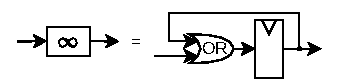
\includegraphics[width=.9\columnwidth]{figures/stickyone/stickyone.pdf}
    \end{center}
    \vspace*{-1em}
    \caption{Sticky-one operator. The sticky-one is reset to zero (not illustrated in the figure) and sticks to 1 once it is set.}
    \label{fig:stickyone}
    \vspace*{-.4em}
\end{figure}


\begin{figure}
    \begin{center}
    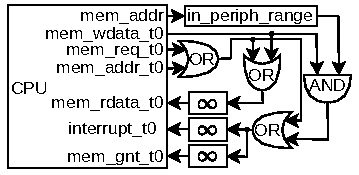
\includegraphics[width=.9\columnwidth]{figures/picinstrum_taints/picinstrum_taints.pdf}
    \end{center}
    \vspace*{-1em}
    \caption{\Pici for a design whose information flows are tracked with dynamic information flow tracking instrumentation. Signals that end with \texttt{t0} represent the taint signals~\cite{tiwari2009complete,solt2022cellift}.
    }
    \label{fig:pic_instrum_taints}
    \vspace*{-.4em}
\end{figure}

\begin{figure}
    \begin{center}
    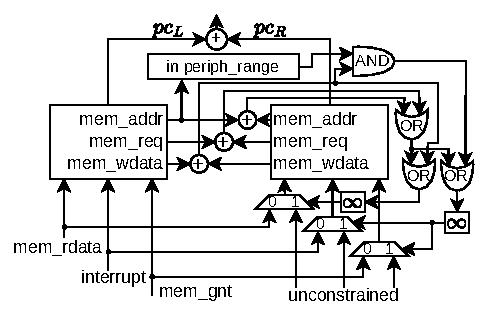
\includegraphics[width=1\columnwidth]{figures/picinstrum_miter/picinstrum_miter.pdf}
    \end{center}
    \vspace*{-1em}
    \caption{\Pici for a design whose information flows are tracked with a miter. }
    \label{fig:pic_instrum_miter}
    \vspace*{-.4em}
\end{figure}

\para{\Pic instrumentation}
We show that such contracts can be expressed as a synthesizable \pici (\PICI).
Because it is an information flow property, the \PICI cannot be directly applied to the CPU under verification (in the original CPU before IFT instrumentation or miter construct, the notion of taint~\cite{solt2022cellift,ceesay2024mucfi} or two-trace property~\cite{wang2023specification,dinesh2024conjunct,dinesh2024conjunct,tan2025contractshadowlogic} does not yet exist).
Instead, the \PICI is applied to the construct that supports information flows, which is either a circuit with dynamic information flow tracking instrumentation, or a miter (see Section~\ref{subsec:ift}).
Before we construct the \PICI, we introduce the sticky-one operator in Figure~\ref{fig:stickyone}, whose functionality is to stay at one as soon as it is set to one, and only comes back to zero when the system is reset.
This operator will model the diamond $\lozenge$ operator in the instrumentations.

We first construct the \PICI for CPUs instrumented for dynamic information flow tracking~\cite{tiwari2009complete,solt2022cellift}.
A contract information flow from a CPU output to a CPU input can be immediately expressed as a wire between the two signals' corresponding taint signals, separated by a sticky-one operator to accommodate for information flows that might return later (i.e., to accommodate for the $\lozenge$ operator).
When several CPU outputs have a contract information flow to a single CPU input, the corresponding taint signals can be combined using a logical OR operation, meaning that the input can be influenced by any of these outputs.
The \PICI for the contract in Equation~\ref{dict:contract_cache_interrupt_addressdependent} is shown in Figure~\ref{fig:pic_instrum_taints} when relying on dynamic information flow tracking instrumentation.
\fls{TODO Check consistency between DIFT and TT}

To construct the \PICI for Equation~\ref{dict:contract_cache_interrupt_addressdependent} for a CPU that relies on a miter construct, the \PICI must ensure that the CPU inputs that are influenced by the CPU outputs are distinct between the two copies of the CPU.
This is achieved using \texttt{XOR} operations between the CPU outputs of the two copies.
Ultimately, another \texttt{XOR} operation with the result of this difference is performed with the input, deciding whether for a given input, the two copies of the CPU will receive the same input, or one copy will receive a flipped input.
Note that there is no conceptual difference between the \PICI for a miter construct and the \PICI for a dynamic information flow tracking instrumentation, yet the latter benefits from the abstraction built into the dynamic information flow tracking instrumentation, which allows for a more compact and arguably more intuitive \PICI.

\para{Take-away}
In Section~\ref{sec:eval}, we will show that when instrumented with the \PICI, the techniques that were originally unable to detect basic timing side-channels due to the verification scope not including caches are now able to detect them.
Importantly, this requires no change to the verification technique implementation at all, as the \PICI becomes part of the design under verification's taint tracking logic or miter construct from the verification tool's perspective.
In terms of performance, we will also show that adding the \PICI incurs a negligible overhead.
However, while the \PICI addresses a necessary condition for maintaining soundness when the CPU under verification is integrated in a system, existing automated constant-time verification tools have other critical shortcomings that affect unsoundness besides platform integration, as we show next in Section~\ref{sec:techniques}.
